\documentclass[letterpaper,10pt]{article}
\usepackage[top=2cm,left=2cm,right=2cm,bottom=3cm]{geometry}

\usepackage{tikz}

\usepackage{multicol}

\usepackage{amsmath}

\setlength{\parskip}{2em}
\setlength{\parindent}{0em}

\renewcommand\thepage{}

\begin{document}

\begin{multicols}{2}

\section*{Líneas rectas}

\textbf{Ejemplo básico}

Hola soy Rodrigo
\begin{tikzpicture}[scale=0.5]
  \draw (0,0) -- (2,0) -- (3,3);
\end{tikzpicture}

\begin{tikzpicture}
  \draw (0,0) -- (2,0) -- (3,3) -- (1,4) -- cycle;
  \draw (0,-1) -- (3,-2);
\end{tikzpicture}


\begin{tikzpicture}
  \draw (0,0) |- (2,2); 
  \draw (0,0) -| (2,2); 
\end{tikzpicture}


\section*{Trayectorias curvas}

\textbf{Curvas de Bezier}

\begin{tikzpicture}
  \draw (0,0) .. controls (2,2) .. (4,0) .. controls(5,-1) .. (6,0);
\end{tikzpicture}

\begin{tikzpicture}
  \draw (0,0) to (3,2);
  \draw (0,0) to[bend right] (3,2);
  \draw (0,0) to[out=120, in=30] (3,2);
\end{tikzpicture}


\begin{tikzpicture}
  \filldraw[fill=green!20,draw=green!40] (0,0) rectangle (2,1);
  \shade[top color=yellow, bottom color=black] (3,0) rectangle (6,2);
\end{tikzpicture}

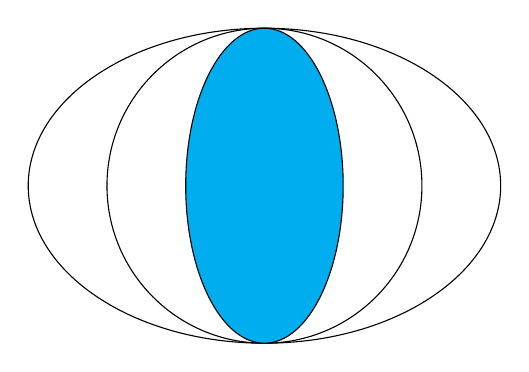
\begin{tikzpicture}
  \draw (0,0) circle [radius=2];
  \draw (0,0) circle [x radius=3, y radius=2];
  \filldraw[fill=cyan] (0,0) ellipse (1 and 2);
\end{tikzpicture}

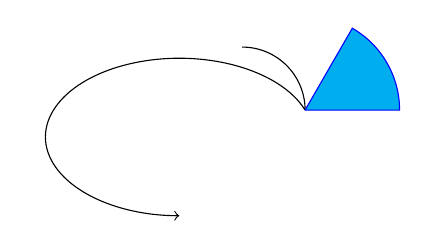
\begin{tikzpicture}
  \draw (0,0) arc (0:90:8mm);
  \draw[->] (0,0) arc (20:270:1.7cm and 1cm);
  \filldraw[fill=cyan, draw=blue] (0,0) -- (12mm,0mm) arc (0:60:12mm) -- (0,0);
\end{tikzpicture}

\begin{tikzpicture}
  \draw[help lines] (0,0) grid (3.9,3.9);
\end{tikzpicture}

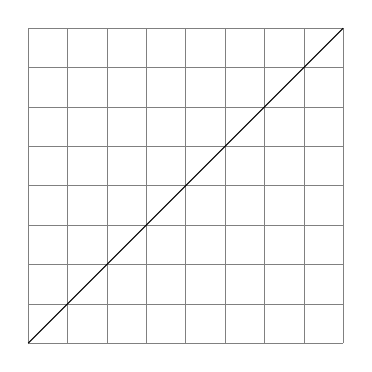
\begin{tikzpicture}
  \draw[step=0.5,gray, very thin] (0,0) grid (4,4);
  \draw (0,0) -- (4,4);
\end{tikzpicture}

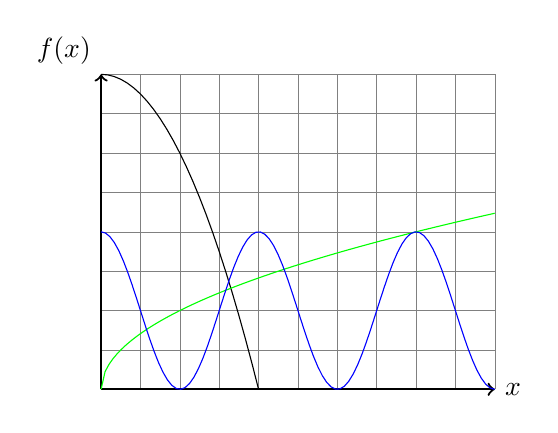
\begin{tikzpicture}
  \draw[step=0.5,gray, very thin] (0,0) grid (5,4);
  \draw[->,thick] (0,0) -- (0,4) node[above=3mm, left]{$f(x)$};
  \draw[->,thick] (0,0) -- (5,0) node[right]{$x$};

  \draw[domain=0:2] plot (\x,{4-\x*\x});
  \draw[domain=0:5,green,samples=100] plot (\x,{sqrt(\x)});
  \draw[domain=0:5,blue,samples=90] plot (\x,{1+cos(pi*\x r)});
\end{tikzpicture}

\begin{tikzpicture}
  \draw[dotted] (0,0) node[below]{n1} -- (1,1) node[right]{n2} -- (0,2)
  node[left]{n3};
\end{tikzpicture}

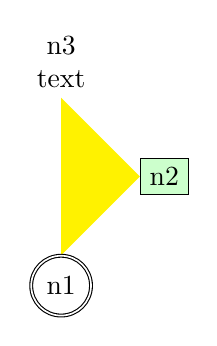
\begin{tikzpicture}
  \fill[fill=yellow] 
  (0,0) node[below,double,circle,draw]{n1} -- 
  (1,1) node[right,rectangle,draw,fill=green!20]{n2} -- 
  (0,2) node[above,align=center]{n3\\text};
\end{tikzpicture}

\begin{tikzpicture}
  %\path (0,0) node(x) {} (3,1) node(y) {};
  \coordinate (x) at (0,0);
  \coordinate (y) at (3,1);
  \draw (x) -- (y);
\end{tikzpicture}

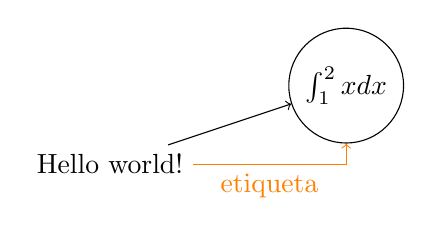
\begin{tikzpicture}
  \path (0,0) node(x){Hello world!}
  (3,1) node[circle,draw](y){$\int_1^2 x d x$};
  \draw[->] (x) -- (y);
  \draw[->,orange]  (x) -| node[below, near start]{etiqueta} (y);
\end{tikzpicture}

\end{multicols}

\end{document}
